\documentclass[]{article}
\usepackage[T1]{fontenc}
\usepackage{lmodern}
\usepackage{amssymb,amsmath}
\usepackage{ifxetex,ifluatex}
\usepackage{fixltx2e} % provides \textsubscript
% use upquote if available, for straight quotes in verbatim environments
\IfFileExists{upquote.sty}{\usepackage{upquote}}{}
\ifnum 0\ifxetex 1\fi\ifluatex 1\fi=0 % if pdftex
  \usepackage[utf8]{inputenc}
\else % if luatex or xelatex
  \ifxetex
    \usepackage{mathspec}
    \usepackage{xltxtra,xunicode}
  \else
    \usepackage{fontspec}
  \fi
  \defaultfontfeatures{Mapping=tex-text,Scale=MatchLowercase}
  \newcommand{\euro}{€}
\fi
% use microtype if available
\IfFileExists{microtype.sty}{\usepackage{microtype}}{}
\usepackage{color}
\usepackage{fancyvrb}
\newcommand{\VerbBar}{|}
\newcommand{\VERB}{\Verb[commandchars=\\\{\}]}
\DefineVerbatimEnvironment{Highlighting}{Verbatim}{commandchars=\\\{\}}
% Add ',fontsize=\small' for more characters per line
\newenvironment{Shaded}{}{}
\newcommand{\KeywordTok}[1]{\textcolor[rgb]{0.00,0.44,0.13}{\textbf{{#1}}}}
\newcommand{\DataTypeTok}[1]{\textcolor[rgb]{0.56,0.13,0.00}{{#1}}}
\newcommand{\DecValTok}[1]{\textcolor[rgb]{0.25,0.63,0.44}{{#1}}}
\newcommand{\BaseNTok}[1]{\textcolor[rgb]{0.25,0.63,0.44}{{#1}}}
\newcommand{\FloatTok}[1]{\textcolor[rgb]{0.25,0.63,0.44}{{#1}}}
\newcommand{\CharTok}[1]{\textcolor[rgb]{0.25,0.44,0.63}{{#1}}}
\newcommand{\StringTok}[1]{\textcolor[rgb]{0.25,0.44,0.63}{{#1}}}
\newcommand{\CommentTok}[1]{\textcolor[rgb]{0.38,0.63,0.69}{\textit{{#1}}}}
\newcommand{\OtherTok}[1]{\textcolor[rgb]{0.00,0.44,0.13}{{#1}}}
\newcommand{\AlertTok}[1]{\textcolor[rgb]{1.00,0.00,0.00}{\textbf{{#1}}}}
\newcommand{\FunctionTok}[1]{\textcolor[rgb]{0.02,0.16,0.49}{{#1}}}
\newcommand{\RegionMarkerTok}[1]{{#1}}
\newcommand{\ErrorTok}[1]{\textcolor[rgb]{1.00,0.00,0.00}{\textbf{{#1}}}}
\newcommand{\NormalTok}[1]{{#1}}
\ifxetex
  \usepackage[setpagesize=false, % page size defined by xetex
              unicode=false, % unicode breaks when used with xetex
              xetex]{hyperref}
\else
  \usepackage[unicode=true]{hyperref}
\fi
\hypersetup{breaklinks=true,
            bookmarks=true,
            pdfauthor={Cezar Ionescu and Patrik Jansson},
            pdftitle={Formal Concept Maps Elements Descriptions (GRACeFUL D4.1)},
            colorlinks=true,
            citecolor=blue,
            urlcolor=blue,
            linkcolor=magenta,
            pdfborder={0 0 0}}
\urlstyle{same}  % don't use monospace font for urls
\setlength{\parindent}{0pt}
\setlength{\parskip}{4pt plus 2pt minus 1pt}
\setlength{\emergencystretch}{3em}  % prevent overfull lines
\setcounter{secnumdepth}{0}

%% Cezar
\usepackage[margin=1.60in]{geometry}
\usepackage[verbose]{wrapfig}
\usepackage{graphicx}
\usepackage{subfig}
\usepackage{rotating}
\usepackage{lscape}
\usepackage{float}
\usepackage{geometry}
\usepackage{framed}
\definecolor{GRACeFULblue}{rgb}{0.20,0.60,0.86}


\author{}
\date{}

\begin{document}

\begin{center}

\includegraphics[width=5cm]{GRACeFULlogo.png}

\textcolor{GRACeFULblue}{Global systems Rapid Assessment tools\\
through Constraint FUnctional Languages}

\vspace{1cm}

FETPROACT-1-2014 Grant Nº 640954

\end{center}

\begin{framed}
\begin{center}
\Large
Formal Concept Maps Elements Descriptions\\[1ex]

D4.1\\[1ex]

\end{center}
\end{framed}

\vspace{1cm}

\noindent
\begin{tabular}{@{}ll@{}}
  Lead Participant:       & Chalmers (Cezar Ionescu, Patrik Jansson)
\\Partners Contributing:  & Deltares, UPC
\\Dissemination Level:    & PU
\\Document Version:       & Final (version 2015-07-24)
\\Date of Submission:     & 2015-07-30
\\Due Date of Delivery:   & 2015-08-01
\end{tabular}

\newpage

\section{Formal Concept Maps Elements
Descriptions}\label{formal-concept-maps-elements-descriptions}

\vfill

\tableofcontents

\vfill

\newpage

\subsection{Abstract}\label{abstract}

This first deliverable of WP4 includes the initial domain modelling:
concept map examples relevant for the CRUD case study, examination and
decomposition of these concept maps into the key underlying elements,
and a formal description of these concept map elements in terms of types
and relations, expressed in a Haskell-like formalism.

\subsection{1. Introduction}\label{introduction}

This document represents the first deliverable of Work Package 4 and is
organised as follows. The first two sections establish the larger
computing science context and the specific notation of the work,
providing brief pointers to functional programming and domain-specific
languages (DSLs).

Section 4 provides a broad picture of the GRACeFUL project and its
relation to policy analysis. An important element of the GRACeFUL system
is the kind of concept map that is used to define the policy problem to
be solved. This is presented in Section 5, together with two examples
resulting from case studies conducted within WP 2 under the direction of
Sadie McEvoy (Deltares).

GRACeFUL concept maps are then formalised using a notation close to the
functional programming language
\href{https://www.haskell.org/}{Haskell}; the result is presented in the
last section of the document.

\subsection{2. Functional Programming}\label{functional-programming}

This section and the next are not self-contained. They serve as a
reminder of the introduction to functional programming and DSLs
presented during the GRACeFUL Kick-Off meeting in Delft, and to
establish the notation used in the remaining sections. There are many
introductions to functional programming, we prefer Bird (2014), Bird
(1998), Bird and Wadler (1988), and Hutton (2007) (although sometimes
billed as successive editions, there is surprisingly little overlap in
the first three books, and they are all worth reading). For a canonical
presentation of DSLs from a functional programming perspective, see
Gibbons (2013).

\subsubsection{2.1 The substitution model}\label{the-substitution-model}

In an imperative programming language, there are two kinds of
syntactical phrases, conventionally called ``expressions'' and
``statements''. Typical expressions are arithmetical expressions
(\VERB|\NormalTok{x }\FunctionTok{+} \DecValTok{2}\NormalTok{, n}\FunctionTok{^}\NormalTok{m}|),
boolean expressions
(\VERB|\NormalTok{a }\FunctionTok{&&} \NormalTok{b, not b}|), etc.
Typical statements are the assignment statement (\VERB|\FunctionTok{=}|
or \VERB|\FunctionTok{:=}|), conditional statements
(\VERB|\KeywordTok{if} \FunctionTok{...} \KeywordTok{then} \FunctionTok{...} \KeywordTok{else} \FunctionTok{...}|)
or loops (\VERB|\NormalTok{for, while, }\FunctionTok{...}|). Expressions
are \emph{evaluated}, and statements are \emph{executed}. The results of
evaluating expressions are values, the results of executing statements
are changes in the state of the computation (and of the computer).

Functional programming does away with statements. Instead, we now have
definitions, such as

\begin{Shaded}
\begin{Highlighting}[]
\NormalTok{fac n  }\FunctionTok{=}  \KeywordTok{if} \NormalTok{n }\FunctionTok{==} \DecValTok{0} \KeywordTok{then} \DecValTok{1} \KeywordTok{else} \NormalTok{n }\FunctionTok{*} \NormalTok{fac (n }\FunctionTok{-} \DecValTok{1}\NormalTok{)}
\end{Highlighting}
\end{Shaded}

The computational mechanism is \emph{substitution} (see Abelson,
Sussman, and Sussman (1996), Section 1.1.5): expressions are replaced by
their definitions until no such substitution is possible. For example:

\begin{Shaded}
\begin{Highlighting}[]

    \NormalTok{fac }\DecValTok{2}
\FunctionTok{=}
    \KeywordTok{if} \DecValTok{2} \FunctionTok{==} \DecValTok{0} \KeywordTok{then} \DecValTok{1} \KeywordTok{else} \DecValTok{2} \FunctionTok{*} \NormalTok{fac (}\DecValTok{2} \FunctionTok{-} \DecValTok{1}\NormalTok{)}
\FunctionTok{=}
    \DecValTok{2} \FunctionTok{*} \NormalTok{fac (}\DecValTok{2} \FunctionTok{-} \DecValTok{1}\NormalTok{)}
\FunctionTok{=}
    \DecValTok{2} \FunctionTok{*} \NormalTok{fac }\DecValTok{1}
\FunctionTok{=}
    \DecValTok{2} \FunctionTok{*} \KeywordTok{if} \DecValTok{1} \FunctionTok{==} \DecValTok{0} \KeywordTok{then} \DecValTok{1} \KeywordTok{else} \DecValTok{1} \FunctionTok{*} \NormalTok{fac (}\DecValTok{1} \FunctionTok{-} \DecValTok{1}\NormalTok{)}
\FunctionTok{=}
    \DecValTok{2} \FunctionTok{*} \DecValTok{1} \FunctionTok{*} \NormalTok{fac (}\DecValTok{1} \FunctionTok{-} \DecValTok{1}\NormalTok{)}
\FunctionTok{=}
    \DecValTok{2} \FunctionTok{*} \DecValTok{1} \FunctionTok{*} \NormalTok{fac }\DecValTok{0}
\FunctionTok{=}
    \DecValTok{2} \FunctionTok{*} \DecValTok{1} \FunctionTok{*} \KeywordTok{if} \DecValTok{0} \FunctionTok{==} \DecValTok{0} \KeywordTok{then} \DecValTok{1} \KeywordTok{else} \DecValTok{0} \FunctionTok{*} \NormalTok{fac (}\DecValTok{0} \FunctionTok{-} \DecValTok{1}\NormalTok{)}
\FunctionTok{=}
    \DecValTok{2} \FunctionTok{*} \DecValTok{1} \FunctionTok{*} \DecValTok{1}
\FunctionTok{=}
    \DecValTok{2}
\end{Highlighting}
\end{Shaded}

It is easy to understand the substitution model intuitively, but it is
hard to give a rigorous description of it. For details, see Peyton Jones
(1987), Section 2.2.

To tackle a programming problem in the imperative setting, we set up an
explicit sequence of states of the computer; the solution is read off
the last state in the sequence. In the functional programming context,
we set up a (potentially very complex) expression with the help of
definitions; the answer is given by evaluating the expression using the
substitution model.

\subsubsection{2.2 Types}\label{types}

Modern functional programming languages are strongly typed, and each
valid expression must have a definite type which can be checked (or even
inferred) at compile time. A new type is introduced by the keyword
\VERB|\KeywordTok{data}| and by rules that tell us how its elements are
constructed. For example:

\begin{Shaded}
\begin{Highlighting}[]
\KeywordTok{data} \DataTypeTok{Day}  \FunctionTok{=}  \DataTypeTok{Monday} \FunctionTok{|} \DataTypeTok{Tuesday} \FunctionTok{|} \DataTypeTok{Wednesday} \FunctionTok{|}
             \DataTypeTok{Thursday} \FunctionTok{|} \DataTypeTok{Friday} \FunctionTok{|} \DataTypeTok{Saturday} \FunctionTok{|} \DataTypeTok{Sunday}
\end{Highlighting}
\end{Shaded}

introduces the set \VERB|\DataTypeTok{Day}| whose values are the labels
\VERB|\DataTypeTok{Monday}\NormalTok{, }\DataTypeTok{Tuesday}\NormalTok{, }\FunctionTok{...}|.

Infinite types are constructed by recursion:

\begin{Shaded}
\begin{Highlighting}[]
\KeywordTok{data} \DataTypeTok{Nat}  \FunctionTok{=}  \DataTypeTok{Z} \FunctionTok{|} \DataTypeTok{S} \DataTypeTok{Nat}
\end{Highlighting}
\end{Shaded}

This definition tells us that a natural number is either just the label
\VERB|\DataTypeTok{Z}|, or the label \VERB|\DataTypeTok{S}| preceding a
natural number. In other words, it is the set
\VERB|\NormalTok{\{}\DataTypeTok{Z}\NormalTok{, }\DataTypeTok{S} \DataTypeTok{Z}\NormalTok{, }\DataTypeTok{S} \NormalTok{(}\DataTypeTok{S} \DataTypeTok{Z}\NormalTok{), }\DataTypeTok{S} \NormalTok{(}\DataTypeTok{S} \NormalTok{(}\DataTypeTok{S} \DataTypeTok{Z}\NormalTok{)), }\ldots\NormalTok{\}}|.
Mathematicians might prefer the representation
\VERB|\NormalTok{\{}\DataTypeTok{Z}\NormalTok{, (}\DataTypeTok{S}\NormalTok{, }\DataTypeTok{Z}\NormalTok{), (}\DataTypeTok{S}\NormalTok{, (}\DataTypeTok{S}\NormalTok{, }\DataTypeTok{Z}\NormalTok{)), }\ldots\NormalTok{\}}|,
which makes it clear that we are only dealing with tuples of labels.
This representation is also close to the way the computer represents
inductive types (Peyton Jones 1987, chap. 10).

New types can be constructed starting from existing ones, for example:

\begin{Shaded}
\begin{Highlighting}[]
\KeywordTok{data} \DataTypeTok{Maybe} \NormalTok{a  }\FunctionTok{=}  \DataTypeTok{Nothing}  \FunctionTok{|}  \DataTypeTok{Just} \NormalTok{a}
\end{Highlighting}
\end{Shaded}

introduces, for any set \VERB|\NormalTok{a}|, the set
\VERB|\DataTypeTok{Maybe} \NormalTok{a }\FunctionTok{=} \NormalTok{\{}\DataTypeTok{Nothing}\NormalTok{\} }\OtherTok{`join`} \NormalTok{\{(}\DataTypeTok{Just}\NormalTok{, x) }\FunctionTok{\VerbBar{}} \NormalTok{x elem a\}}|.
This is a standard datatype, allowing us to model partiality, and will
be used below.

Types are one of the most important tools for writing specifications. In
particular, most programs will have a \emph{function type}

\begin{Shaded}
\begin{Highlighting}[]
program \OtherTok{::} \DataTypeTok{Input} \OtherTok{->} \DataTypeTok{Output}
\end{Highlighting}
\end{Shaded}

An expressive type system allows us to conclude many facts about
\VERB|\NormalTok{program}| from its type.

An important information about a type is its \emph{name}. The sets of
values used to model credit and debit are the same, but whether a given
value is to be interpreted in one way or in the other can make a great
deal of difference. So we would like to say

\begin{Shaded}
\begin{Highlighting}[]
\DataTypeTok{Credit}  \FunctionTok{=}  \DataTypeTok{Real}
\DataTypeTok{Debit}   \FunctionTok{=}  \DataTypeTok{Real}
\end{Highlighting}
\end{Shaded}

but the symbol \VERB|\FunctionTok{=}| can only be used with expressions.
To avoid confusion, Haskell uses the keyword \VERB|\KeywordTok{type}|:

\begin{Shaded}
\begin{Highlighting}[]
\KeywordTok{type} \DataTypeTok{Credit}  \FunctionTok{=}  \DataTypeTok{Real}
\KeywordTok{type} \DataTypeTok{Debit}   \FunctionTok{=}  \DataTypeTok{Real}
\end{Highlighting}
\end{Shaded}

We will make use of this ability to introduce new names for the same
type below.

\subsubsection{2.3 Type classes and
polymorphism}\label{type-classes-and-polymorphism}

Types allow us to organise the universe of values. It is often useful to
organise the universe of types as well. For example, the only types that
can be used to represent qualitative values are types that can be
\emph{linearly ordered}, i.e., for which we can tell, for any two
values, whether they are equal, and if not, which is smaller and which
is bigger. Natural numbers are like that, functions are not.

Different functional programming languages offer different mechanisms
for organising types. Haskell has \emph{type classes}. The type class
\VERB|\DataTypeTok{Ord}|, which we'll use below, is introduced by

\begin{Shaded}
\begin{Highlighting}[]
\KeywordTok{class} \DataTypeTok{Eq} \NormalTok{a }\OtherTok{=>} \DataTypeTok{Ord} \NormalTok{a }\KeywordTok{where}
   \NormalTok{(}\FunctionTok{<}\NormalTok{), (}\FunctionTok{<=}\NormalTok{), (}\FunctionTok{>=}\NormalTok{), (}\FunctionTok{>}\NormalTok{)  }\OtherTok{::} \NormalTok{a }\OtherTok{->} \NormalTok{a }\OtherTok{->} \DataTypeTok{Bool}
\end{Highlighting}
\end{Shaded}

This tells us that a set \VERB|\NormalTok{a}| can only be ordered if its
values can be compared for equality
(\VERB|\DataTypeTok{Eq} \NormalTok{a}|). Further, in order for
\VERB|\NormalTok{a}| to qualify as an \emph{instance} of
\VERB|\DataTypeTok{Ord}|, we must have defined the standard comparison
functions for it.

Some functional expressions can be evaluated no matter what the type of
the argument to which they are applied. For example, the identity
function is defined by

\begin{Shaded}
\begin{Highlighting}[]
\NormalTok{id x  }\FunctionTok{=}  \NormalTok{x}
\end{Highlighting}
\end{Shaded}

This equation defines, for every type \VERB|\DataTypeTok{A}|, a function
\VERB|idA \OtherTok{::} \DataTypeTok{A} \OtherTok{->} \DataTypeTok{A}|.
Thus, \VERB|\NormalTok{id}| itself is a template for creating such
functions, one for each type. Such template-like functions are called
\emph{polymorphic}. In Haskell typings, lower-case variables denote
universally quantified variables. For example:

\begin{Shaded}
\begin{Highlighting}[]
\NormalTok{id}\OtherTok{  ::}  \NormalTok{a }\OtherTok{->} \NormalTok{a}
\end{Highlighting}
\end{Shaded}

is read: ``for every type \VERB|\NormalTok{a}|, there exists a function
\VERB|\NormalTok{id}\OtherTok{ ::} \NormalTok{a }\OtherTok{->} \NormalTok{a}|''.

Type classes allow a more refined form of polymorphism. For example, the
equation

\begin{Shaded}
\begin{Highlighting}[]
\NormalTok{max x y  }\FunctionTok{=}  \KeywordTok{if} \NormalTok{x }\FunctionTok{<} \NormalTok{y }\KeywordTok{then} \NormalTok{y }\KeywordTok{else} \NormalTok{x}
\end{Highlighting}
\end{Shaded}

defines a function \VERB|\NormalTok{max}| for all the types whose values
we can compare with \VERB|\FunctionTok{<}|. Thus, a typing such as
\VERB|\NormalTok{a }\OtherTok{->} \NormalTok{a }\OtherTok{->} \NormalTok{a}|
would be too general, one such as
\VERB|\DataTypeTok{Int} \OtherTok{->} \DataTypeTok{Int} \OtherTok{->} \DataTypeTok{Int}|
too specific. The type class \VERB|\DataTypeTok{Ord}| allows us to
\emph{constrain} the polymorphism of \VERB|\NormalTok{max}|:

\begin{Shaded}
\begin{Highlighting}[]
\NormalTok{max}\OtherTok{  ::}  \DataTypeTok{Ord} \NormalTok{a }\OtherTok{=>} \NormalTok{a }\OtherTok{->} \NormalTok{a }\OtherTok{->} \NormalTok{a}
\end{Highlighting}
\end{Shaded}

This is read: ``for every type \VERB|\NormalTok{a}| that is a member of
the type class \VERB|\DataTypeTok{Ord}|, \VERB|\NormalTok{max}| is a
function of type
\VERB|\NormalTok{a }\OtherTok{->} \NormalTok{a }\OtherTok{->} \NormalTok{a}|''.

\subsection{3. Domain-Specific
Languages}\label{domain-specific-languages}

Suppose we want to count the number of floating-point multiplications
performed by a program. Since the built-in floating-point operations do
not keep track of this information, we have to replace them with ones
that do. A possible way of doing that is:

\begin{Shaded}
\begin{Highlighting}[]
\KeywordTok{type} \DataTypeTok{CDouble} \FunctionTok{=} \NormalTok{(}\DataTypeTok{Double}\NormalTok{, }\DataTypeTok{Int}\NormalTok{)}

mkCDouble  \OtherTok{::}  \DataTypeTok{Double}   \OtherTok{->}  \DataTypeTok{CDouble}
add        \OtherTok{::}  \DataTypeTok{CDouble}  \OtherTok{->}  \DataTypeTok{CDouble}  \OtherTok{->}  \DataTypeTok{CDouble}
mul        \OtherTok{::}  \DataTypeTok{CDouble}  \OtherTok{->}  \DataTypeTok{CDouble}  \OtherTok{->}  \DataTypeTok{CDouble}

\NormalTok{mkCDouble x            }\FunctionTok{=}  \NormalTok{(x, }\DecValTok{0}\NormalTok{)}
\NormalTok{add (x1, n1) (x2, n2)  }\FunctionTok{=}  \NormalTok{(x1}\FunctionTok{+}\NormalTok{x2, n1}\FunctionTok{+}\NormalTok{n2)}
\NormalTok{mul (x1, n1) (x2, n2)  }\FunctionTok{=}  \NormalTok{(x1}\FunctionTok{*}\NormalTok{x2, n1}\FunctionTok{+}\NormalTok{n2}\FunctionTok{+}\DecValTok{1}\NormalTok{)}
\end{Highlighting}
\end{Shaded}

For simplicity, we have only shown the addition and multiplication
operations. These new operations will act on ``counted doubles'',
members of the type \VERB|\DataTypeTok{CDouble}|, represented by pairs
that consist of the actual value and the number of multiplications
required to produce it. Thus, we need a way of turning ordinary doubles
into counted doubles, which is achieved by \VERB|\NormalTok{mkCDouble}|.
We have separated the interface, consisting of the signatures of the
operations, from the implementation, and we hope the example is
straightforward.

Consider now a different problem, that of controlling the round-off
errors in arithmetical operations. One way of achieving that is to work
with \emph{intervals}, rather than point values. Again, we will need to
replace the standard operations with new ones, acting on ``controlled
values'', i.e., intervals represented as pairs of numbers. Again, the
following implementation should be straightforward:

\begin{Shaded}
\begin{Highlighting}[]
\KeywordTok{type} \DataTypeTok{CDouble} \FunctionTok{=} \NormalTok{(}\DataTypeTok{Double}\NormalTok{, }\DataTypeTok{Double}\NormalTok{)}

mkCDouble  \OtherTok{::}  \DataTypeTok{Double}   \OtherTok{->}  \DataTypeTok{CDouble}
add        \OtherTok{::}  \DataTypeTok{CDouble}  \OtherTok{->}  \DataTypeTok{CDouble}  \OtherTok{->}  \DataTypeTok{CDouble}
mul        \OtherTok{::}  \DataTypeTok{CDouble}  \OtherTok{->}  \DataTypeTok{CDouble}  \OtherTok{->}  \DataTypeTok{CDouble}

\NormalTok{mkCDouble x            }\FunctionTok{=}  \NormalTok{(x, x)}
\NormalTok{add (xl, xu) (yl, yu)  }\FunctionTok{=}  \NormalTok{(xl}\FunctionTok{+}\NormalTok{yl, xu}\FunctionTok{+}\NormalTok{yu)}
\NormalTok{mul (xl, xu) (yl, yu)  }\FunctionTok{=}  \NormalTok{(lb, ub)}
  \KeywordTok{where}
  \NormalTok{lb  }\FunctionTok{=}  \NormalTok{minimum [xl }\FunctionTok{*} \NormalTok{yl, xl }\FunctionTok{*} \NormalTok{yu, xu }\FunctionTok{*} \NormalTok{yl, xu }\FunctionTok{*} \NormalTok{yu]}
  \NormalTok{ub  }\FunctionTok{=}  \NormalTok{maximum [xl }\FunctionTok{*} \NormalTok{yl, xl }\FunctionTok{*} \NormalTok{yu, xu }\FunctionTok{*} \NormalTok{yl, xu }\FunctionTok{*} \NormalTok{yu]}
\end{Highlighting}
\end{Shaded}

You will notice that the interface is exactly the same as in the
previous case. This points to a code duplication problem: we are doing
the same work twice. Most software engineering methodologies, such as
structural programming, object-oriented programming, or DSLs, can be
understood as attempts at solving such problems.

In our case, the object-oriented solution would factor out the
duplicated part by creating an abstract class or an interface. Then, new
classes would be defined for ``counted arithmetic'' and ``controlled
arithmetic'', which would inherit from the abstract class. Code which
does not depend on the kind of arithmetic implemented ``under the hood''
would be written in terms of the abstract class, and thus be polymorphic
with respect to the implementation. This suggests a possible refactoring
in Haskell, by introducing a type class for the abstract arithmetic.

The DSL solution is somewhat different. It starts by recognising that
the common part represents the \emph{syntax} of arithmetical
expressions, and makes this explicit by introducing a datatype for these
expressions:

\begin{Shaded}
\begin{Highlighting}[]
\KeywordTok{data} \DataTypeTok{CDouble}  \FunctionTok{=}  \DataTypeTok{MkCDouble} \DataTypeTok{Double}
              \FunctionTok{|}  \DataTypeTok{Add} \DataTypeTok{CDouble} \DataTypeTok{CDouble}
              \FunctionTok{|}  \DataTypeTok{Mul} \DataTypeTok{CDouble} \DataTypeTok{CDouble}
\end{Highlighting}
\end{Shaded}

An element of \VERB|\DataTypeTok{CDouble}| is just a syntactical piece
of data, such as

\begin{Shaded}
\begin{Highlighting}[]
       \DataTypeTok{Add} \NormalTok{(}\DataTypeTok{MkCDouble} \FloatTok{2.0}\NormalTok{) (}\DataTypeTok{Mul} \NormalTok{(}\DataTypeTok{MkCDouble} \FloatTok{3.5}\NormalTok{) (}\DataTypeTok{MkCDouble} \NormalTok{(}\FunctionTok{-}\FloatTok{1.2}\NormalTok{)))}
\end{Highlighting}
\end{Shaded}

or, in more familiar notation,
\VERB|\FloatTok{2.0} \FunctionTok{+} \FloatTok{3.5} \FunctionTok{*} \NormalTok{(}\FunctionTok{-}\FloatTok{1.2}\NormalTok{)}|.

The various kinds of arithmetic give these syntactical elements
different \emph{semantics} or interpretations. There exists a
\emph{semantic domain}
(\VERB|\NormalTok{(}\DataTypeTok{Double}\NormalTok{, }\DataTypeTok{Int}\NormalTok{)}|
in the case of counted values,
\VERB|\NormalTok{(}\DataTypeTok{Double}\NormalTok{, }\DataTypeTok{Double}\NormalTok{)}|
in that of controlled values); the expressions will be evaluated to
elements of this domain. In addition to the semantic domain, every
interpretation will need functions that evaluate the basic forms of
arithmetical expressions: \VERB|\DataTypeTok{MkCDouble} \NormalTok{x}|,
\VERB|\DataTypeTok{Add} \NormalTok{x y}|, and
\VERB|\DataTypeTok{Mul} \NormalTok{x y}|. Thus, an interpretation is
defined by a type and three functions:

\begin{Shaded}
\begin{Highlighting}[]
\KeywordTok{type} \DataTypeTok{CAlg} \NormalTok{a  }\FunctionTok{=}  \NormalTok{(}\DataTypeTok{Double} \OtherTok{->} \NormalTok{a,}
                 \NormalTok{a }\OtherTok{->} \NormalTok{a }\OtherTok{->} \NormalTok{a,}
                 \NormalTok{a }\OtherTok{->} \NormalTok{a }\OtherTok{->} \NormalTok{a)}

\CommentTok{-- "Helper" functions:}
\NormalTok{mk (f, g, h)   }\FunctionTok{=}  \NormalTok{f}
\NormalTok{a  (f, g, h)   }\FunctionTok{=}  \NormalTok{g}
\NormalTok{m  (f, g, h)   }\FunctionTok{=}  \NormalTok{h}
\end{Highlighting}
\end{Shaded}

In other words, an interpretation is given by an \emph{algebra} (in the
sense of \emph{universal algebra}).

The \emph{evaluation} of syntactical expressions in a specific algebra
can now be implemented \emph{generically}, as a \emph{homomorphism}:

\begin{Shaded}
\begin{Highlighting}[]
eval \OtherTok{::} \DataTypeTok{CDouble} \OtherTok{->}  \DataTypeTok{CAlg} \NormalTok{a  }\OtherTok{->} \NormalTok{a}
\NormalTok{eval (}\DataTypeTok{MkCDouble} \NormalTok{x)  alg     }\FunctionTok{=}  \NormalTok{mk alg x}
\NormalTok{eval (}\DataTypeTok{Add} \NormalTok{x1 x2)    alg     }\FunctionTok{=}  \NormalTok{a alg (eval x1 alg) (eval x2 alg)}
\NormalTok{eval (}\DataTypeTok{Mul} \NormalTok{x1 x2)    alg     }\FunctionTok{=}  \NormalTok{m alg (eval x1 alg) (eval x2 alg)}
\end{Highlighting}
\end{Shaded}

The various kinds of arithmetic are then represented by different
algebras:

\begin{Shaded}
\begin{Highlighting}[]
countAlg  \OtherTok{::}  \DataTypeTok{CAlg} \NormalTok{(}\DataTypeTok{Double}\NormalTok{, }\DataTypeTok{Int}\NormalTok{)}
\NormalTok{countAlg   }\FunctionTok{=}  \NormalTok{(mk, a, m) }\KeywordTok{where}
  \NormalTok{mk x                 }\FunctionTok{=}  \NormalTok{(x, }\DecValTok{0}\NormalTok{)}
  \NormalTok{a (x1, n1) (x2, n2)  }\FunctionTok{=}  \NormalTok{(x1}\FunctionTok{+}\NormalTok{x2, n1}\FunctionTok{+}\NormalTok{n2)}
  \NormalTok{m (x1, n1) (x2, n2)  }\FunctionTok{=}  \NormalTok{(x1}\FunctionTok{*}\NormalTok{x2, n1}\FunctionTok{+}\NormalTok{n2}\FunctionTok{+}\DecValTok{1}\NormalTok{)}

controlAlg  \OtherTok{::}  \DataTypeTok{CAlg} \NormalTok{(}\DataTypeTok{Double}\NormalTok{, }\DataTypeTok{Double}\NormalTok{)}
\NormalTok{controlAlg   }\FunctionTok{=}  \NormalTok{(mk, a, m) }\KeywordTok{where}
  \NormalTok{mk x                 }\FunctionTok{=}  \NormalTok{(x, x)}
  \NormalTok{a (xl, xu) (yl, yu)  }\FunctionTok{=}  \NormalTok{(xl}\FunctionTok{+}\NormalTok{yl, xu}\FunctionTok{+}\NormalTok{yu)}
  \NormalTok{m (xl, xu) (yl, yu)  }\FunctionTok{=}  \NormalTok{(lb, ub)}
    \KeywordTok{where}
    \NormalTok{lb  }\FunctionTok{=}  \NormalTok{minimum [xl }\FunctionTok{*} \NormalTok{yl, xl }\FunctionTok{*} \NormalTok{yu, xu }\FunctionTok{*} \NormalTok{yl, xu }\FunctionTok{*} \NormalTok{yu]}
    \NormalTok{ub  }\FunctionTok{=}  \NormalTok{maximum [xl }\FunctionTok{*} \NormalTok{yl, xl }\FunctionTok{*} \NormalTok{yu, xu }\FunctionTok{*} \NormalTok{yl, xu }\FunctionTok{*} \NormalTok{yu]}
\end{Highlighting}
\end{Shaded}

In brief, the DSL approach starts by making explicit the syntax of the
problem domain and the various semantical interpretations of this
syntax. Almost always\footnote{For an analysis of the reach of this
  scheme, and the reasons for it, see Gibbons and Wu (2014).}, the
syntax is implemented as an inductive data type parametrised over the
semantical domains, the semantics is given by an algebra, evaluation is
a homomorphism of algebras, and the various applications are represented
by particular algebras.

These algebras are equivalent to the classes of the object-oriented
solution. Therefore, the DSL approach is somewhat ``heavier'', it needs
a larger up-front investment. However, it is also more flexible: it
makes a distinction between the applications that need only work with
the \emph{syntax} of expressions (such as parsers or pretty-printers),
those that need to work only with the \emph{semantics} (as in the case
of our original tasks, counting multiplications or controlling round-off
errors), and applications that need both (such as compilers and other
forms of translation, or applications that need to mix various
interpretations). Moreover, it offers new ways of understanding a
problem domain, of formalising it, of dividing it into sub-problems, and
of combining the resulting solutions.

\subsection{4. Policy Analysis in the context of
GRACeFUL}\label{policy-analysis-in-the-context-of-graceful}

\emph{Policy analysis} is a method for assisting policymakers in solving
real-world policy problems, involving many stakeholders with conflicting
interests, essential uncertainties, and many overlapping potential
actions. Since its beginnings in the 50s in the world of operations
research, policy analysis has been refined and given several different
formulations. In one influential article, Warren Walker (2000)
summarises the steps of policy analysis in the following way:

\begin{enumerate}
\def\labelenumi{\arabic{enumi}.}
\item
  Identify the problem. Involves identifying the questions or issues
  involved, fixing the context within which the issues are to be
  analysed and the policies will have to function, clarifying
  constraints on possible courses of action, identifying the people who
  will be affected by the policy decision, discovering the major
  operative factors and deciding on the initial approach.
\item
  Identify the objectives of the new policy. Involves formulating the
  objectives that, if met, would solve the policy problem. Usually,
  there will be multiple conflicting objectives.
\item
  Decide on criteria (measures of performance and cost) with which to
  evaluate alternative policies. The criteria must be measurable (but
  note that qualitative values such as ``big'', ``likely'', etc. are
  acceptable). This step also identifies the ways in which the costs of
  the policies are to be estimated.
\item
  Select the alternative policies to be evaluated. A \emph{policy} is
  defined ``loosely'' as ``a set of actions taken to solve a problem'',
  implying that alternative policies are defined in terms of more
  elementary \emph{actions}. As many alternatives should be taken into
  account as possible, and the current policy must be included as ``base
  case''.
\item
  Analyse each alternative. Each alternative must be evaluated in every
  possible future context (scenario). Notice that the choice of
  scenarios which express uncertainty has to be part of the previous
  steps, even though this is not explicitly stated in Walker's article.
  This step involves commissioning external experts, collecting relevant
  data, setting up simulations, etc.
\item
  Compare the alternatives in terms of projected costs and effects. If
  none of the alternatives is good enough, then some or all of the steps
  1-5 have to be re-examined.
\item
  Implement the chosen alternative.
\item
  Monitor and evaluate the results.
\end{enumerate}

There are three major inter-related problems with the kind of procedure
outlined here:

\begin{enumerate}
\def\labelenumi{\alph{enumi}.}
\item
  Perhaps the most important difficulty is the feedback explicitly
  introduced in step 6, after the execution of step 5. Step 5 is one of
  the longest and most expensive pre-implementation steps, since it
  involves external contractors, experts in the fields under
  consideration, and the setting up of potentially long-running computer
  simulations. And yet, at the end of this step, all the work done so
  far can be called into question and need to be redone. Depending on
  the amount of time that step 5 has taken (usually measured in months),
  this might not even be possible. Even if the problem, goals, criteria,
  or alternatives can be redefined, a new step 5 will still be quite
  expensive, both in terms of actual money and of time. And there is no
  guarantee that a second iteration will not result in a third, etc.
\item
  The second problem is that step 4 is error prone. As Walker
  underlines, ``as many alternatives as stand any chance at all of being
  worthwhile'' should be included. An alternative should not be excluded
  ``merely because it seems impractical or runs contrary to past
  practice'', and ``personal judgements on such issues should be
  withheld''. But this advice seems very hard to follow. Many people
  might not even be aware of excluding an alternative because it seems
  impractical and runs against their personal judgement: they will
  simply not consider it at all.
\item
  The third problem is that formulating many alternatives, being forced
  to consider even apparently ``impractical'' ones which ``run contrary
  to past practice'', increases considerably the costs of step 5 (recall
  that every alternative has to be considered in the context of
  \emph{all} future scenarios). Moreover, the more results the
  stakeholders have to consider at the end of step 5, the more difficult
  it will be to present them in a perspicuous, useful manner.
\end{enumerate}

The GRACeFUL system will offer feedback at every point of the problem
definition in steps 1-3, for example by offering a library of criteria
that could be used to assess chosen goals. But its main role will be to
eliminate or alleviate these three problems, which all appear in steps
4-6. The key ideas are:

\begin{itemize}
\item
  Instead of relying on the stakeholders to provide alternative policies
  (sets of atomic actions), they will only be required to provide the
  actions that could go into building the alternatives. This is a much
  easier process, if only for cardinality reasons. The number of
  possible alternatives is always greater than the number of actions,
  since each action can be considered an alternative policy in itself.
  In the worst case, however, in which the actions can be combined
  arbitrarily, there are, for \VERB|\NormalTok{n}| actions, on the order
  of \VERB|\DecValTok{2}\FunctionTok{^}\NormalTok{n}| alternatives! More
  importantly, enumerating the actions is a more objective process than
  selecting alternatives against ``personal judgements'' or ``past
  practices''. The GRACeFUL system will maintain a database of atomic
  actions relevant to the policy problems at hand, in order to make this
  enumeration even easier.
\item
  The question of finding the combinations of actions that fulfil the
  criteria and thus satisfy the desired goals, which was previously a
  matter of ``test-and-rank'', now becomes a matter of problem solving,
  in particular, a matter of \emph{constraint programming}
%
\footnote{
%
  Similarly to functional and logic programming, \emph{constraint
    programming} is a declarative programming paradigm.  The program
  is formulated in terms of a number of constraints, and the
  \emph{constraint solver} identifies the solutions satisfying these
  constraints (there might be none, one, or many such solutions).  For
  more information, see, e.g.,
%
    \href{http://www.constraint.org/en/intro.html}{Constraint.org}.
%
}.
\end{itemize}

\begin{itemize}
\item
  In order to apply constraint programming, however, a suitable
  formulation of the problem is needed. This is achieved by building a
  qualitative or semi-qualitative model on the basis of the problem
  definition obtained from the stakeholders in steps 1-3 and of the list
  of actions. An essential feature of the model is that it will
  incorporate not just the constraints defined by the criteria, but also
  those introduced by relations between actions and factors. For
  example, an action requiring investment is constrained by available
  capital (an example of a factor).
\item
  The qualitative model can then be used by the constraint programming
  layer to

  \begin{enumerate}
  \def\labelenumi{\roman{enumi}.}
  \item
    find alternative policies that can satisfy the goals,
  \item
    identify inconsistencies in the problem definition,
  \item
    present visualisations of possible future trajectories.
  \end{enumerate}
\end{itemize}

A key feature of the GRACeFUL system is that these outputs are
accompanied by \emph{explanations}. For example, the inconsistencies can
be traced down to conflicting goals of stakeholders, resulting in
conflicting criteria. As another example, the users can understand why
certain actions are (or are not) selected.

Since the GRACeFUL system examines the space of \emph{all} possible
alternative policies, the problem of not including relevant alternatives
is eliminated. Since the problem solving process of constraint
programming is using the information supplied by the constraints, it can
be much more effective then a simple ``test-and-rank'' process; thus,
the problem of computational complexity is alleviated.

Additionally, constraint programming makes it possible to solve another
problem that has plagued qualitative simulation systems: the explosion
of possible future trajectories. By using the information provided by
stakeholder goals and preferences, the constraint programming layer will
be able to prune the graph of future trajectories, enabling a useful
presentation of the simulation results.

The constraint programming layer will, however, not interact with the
stakeholders directly. The information from and for the stakeholders
will go through at least two layers of the GRACeFUL system: first,
through the graphical visual interface, which will assist the
stakeholders in building the problem definition, and which will present
the results of the qualitative simulations, and second, the DSLs which
will translate between these interfaces and the constraint programming
layer.

\subsection{5. GRACeFUL Concept Maps}\label{graceful-concept-maps}

We envisage the GRACeFUL process to follow broadly the de Haan and de
Heer framework for solving complex problems ({de Haan} and Heer 2015).
In this process, the result corresponding to steps 1-4 of policy
analysis are presented in the form of a \emph{GRACeFUL concept map}.
This concept map contains all the elements of a policy problem
definition discussed above: goals, criteria for assessing the
achievement of those goals, a description of the system as a causal loop
diagram involving factors and criteria, and the competing alternatives.

The steps leading to a GRACeFUL concept map are to be performed by the
stakeholders, assisted by an expert controlling the GRACeFUL system. For
example, the goals elicited from a stakeholder or groups of stakeholder,
are refined to measurable criteria of achievement of those goals. This
is achieved by discussions, brain storming sessions, etc., but also by
interacting with the GRACeFUL system, which provides a growing library
of criteria that are relevant for a given goal.

Similarly, the description of the system is elicited from stakeholders
with help from the GRACeFUL system, which contains a library of relevant
factors, relating them to the concepts under discussion. Here, the term
\emph{factors} refers to \emph{characteristics of a system that can take
a value, either quantitative or qualitative, that can change over time}
(source: the \emph{GRACeFUL Glossary of Terms}). In mathematical system
theory, a collection of factors correspond to the \emph{state} of the
system. Similarly, \emph{external factors} correspond to \emph{inputs}
to the system. As such, factors are assumed to be associated with
measurable (if only in qualitative terms) values.

As in systems theory, a distinction is made between inputs that are
beyond the control of the system, and which are potentially uncertain
(or even unknown), and \emph{actions} or combinations of actions, which
represent the system theoretical \emph{controls}, generally assumed to
be deterministic but with uncertain consequences.

The interaction between the factors, and between the factors and the
criteria, represents a first description of the system (no alternatives
are present, or only the baseline policy is assumed to be active). This
description is in the form of a \emph{causal loop diagram}. A causal
loop diagram is a form of \emph{directed, simple, labelled graph}, i.e.:

\begin{enumerate}
\def\labelenumi{\alph{enumi}.}
\item
  a link between two nodes has a well-defined source and a target (it is
  \emph{directed}); intuitively, the link represents a causal relation
  between the source (cause) and the target (effect);
\item
  there can be at most one connection from one node to another (the
  graph is \emph{simple}): either a causal relation exists, or it does
  not. Note, however, that since the graph is directed, there may be an
  inverse connection from the ``effect'' to the ``cause'', as in
  feedback loops;
\item
  the connections are either \emph{positive} (an increase in the value
  of the source causes an increase in the value of the target), or
  \emph{negative} (an increase causes a decrease), hence the graph is
  \emph{labelled}.
\end{enumerate}

It can be seen from the last point that nodes \emph{must} represent
values that can be partially ordered. This rules out nodes that
represent, say, stakeholders.

As an example, two such causal loop diagrams, produced in the
student sessions organised as part of the CRUD case study, can be
found in the Appendix.

The GRACeFUL system can assist in building the causal loop diagram, for
example by suggesting connections, or by pointing out inconsistencies.

At this stage, if we can attribute qualitative values to the various
nodes, the causal loop diagram describes a system that can make the
object of a qualitative simulation. The criteria play the roles of
constraints: the qualitative trajectories that lead outside the criteria
can be pruned by the constraint programming system.

The causal loop diagram is enhanced to a GRACeFUL concept map by the
addition of extra nodes and non-causal links. The extra nodes represent
actions, goals, alternatives, and stakeholders.

Like all previous elements, the actions are also obtained from the
stakeholders. As explained in the previous section, actions are the
components of alternatives, among which will be found the policy
solutions we are seeking. Alternatives are, according to the GRACeFUL
Glossary of Terms, ``action or combination of actions that influence the
values of criteria''. They correspond to Walker's ``alternative
policies'', where a \emph{policy} is defined ``loosely'' as ``a set of
actions taken to solve a problem''. As in the case of goal definition,
the GRACeFUL system can suggest such ``atomic actions'' that are useful
to the goals in the context of the problem at hand.

The role of actions in the GRACeFUL concept maps is to give initial
values to the factors and criteria they influence. They do not link via
causal loops to these factors, since actions are not of the requisite
type (they do not represent values that can increase or decrease).
However, they will usually have non-causal links, representing
constraining relationships to the factors.

In the other cases of extra nodes (goals, alternatives, and
stakeholders), the links represent primarily ``belongs to''
relationships: there are links from stakeholders to goals, indicating
which stakeholders have declared which goals; there are links from goals
to the criteria by which they are assessed; finally, there are links
between alternatives and the factors and criteria that they (i.e., their
constituent atomic actions) influence.

Figure \ref{fig:cm} (drawn by Sadie McEvoy (Deltares)) shows a
graphical representation of the structure of a GRACeFUL concept map:

\begin{figure}[!ht]%
  \centering
 {{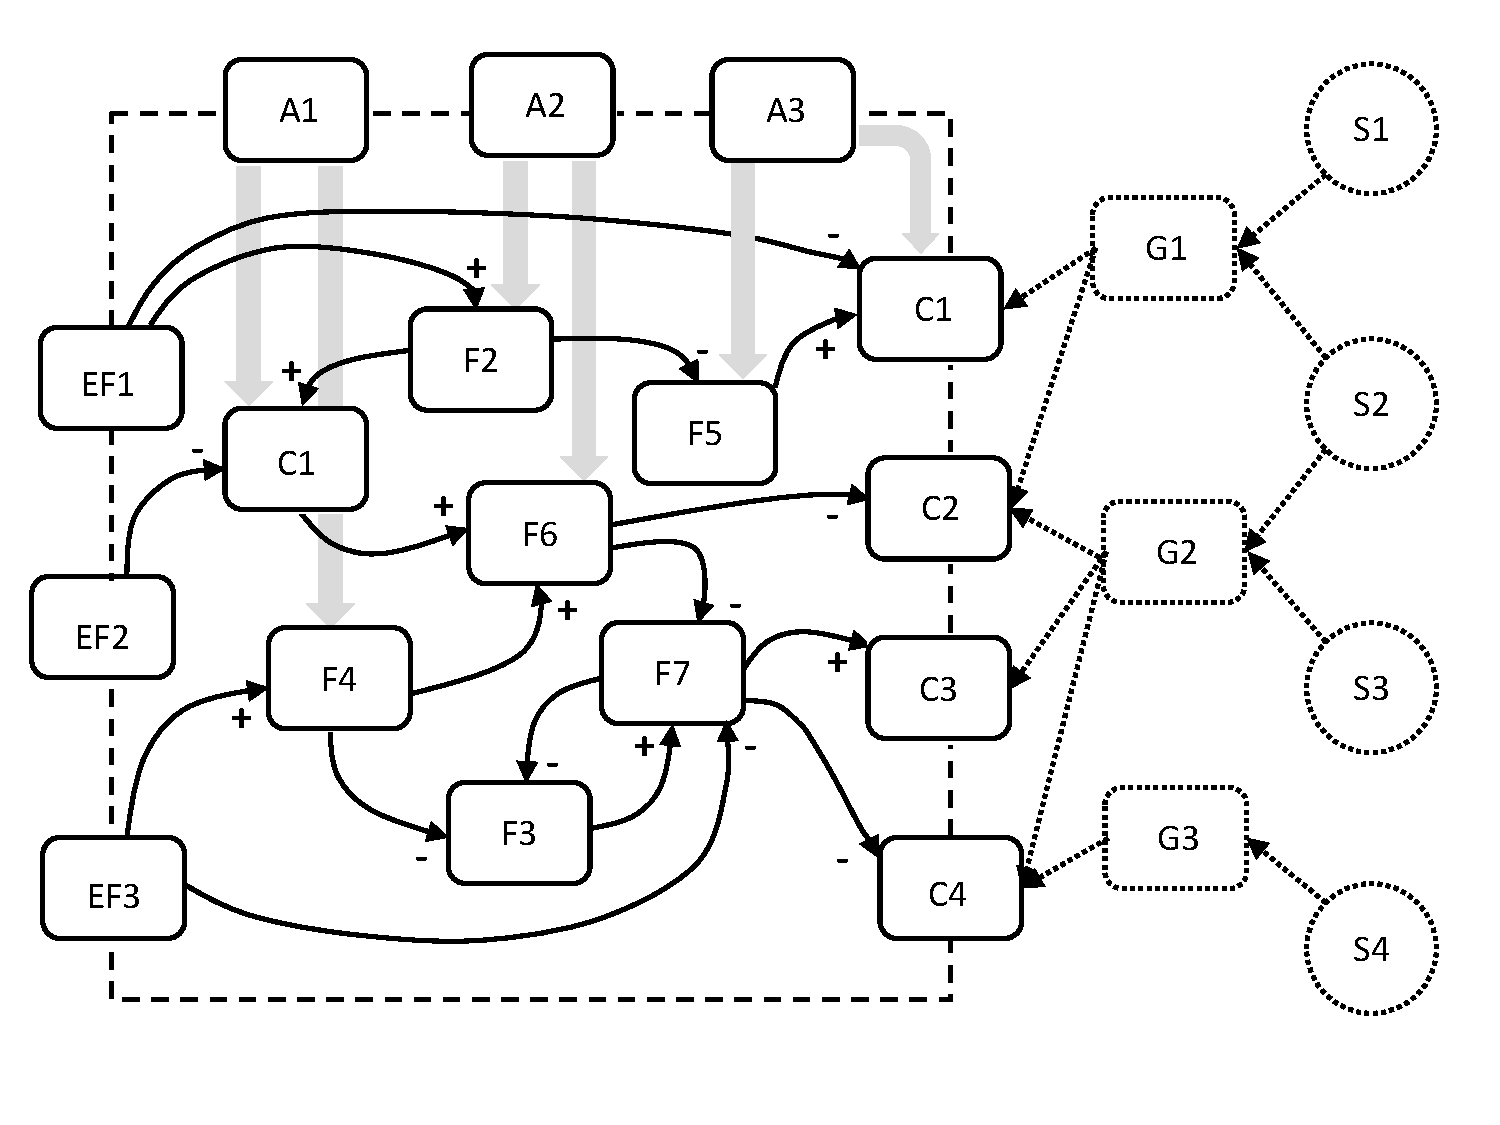
\includegraphics[width=0.9\textwidth]{../s4.pdf} }}%
  \caption{The structure of a GRACeFUL concept map}%
  \label{fig:cm}%
\end{figure}

\subsection{6. Formal Description of GRACeFUL Concept Maps
Elements}\label{formal-description-of-graceful-concept-maps-elements}

We now formalise the structural elements of the GRACeFUL concept maps
presented in the previous section. These elements are:

\begin{itemize}
\itemsep1pt\parskip0pt\parsep0pt
\item
  goals
\item
  criteria
\item
  concepts
\item
  factors
\item
  connections
\item
  stakeholders
\item
  actions
\item
  alternatives
\item
  constraints
\end{itemize}

Let us start with concepts and factors, which are, in a sense, the
simplest elements of the GRACeFUL concept maps. Concepts are high-level
descriptions of the components of a system, and they are refined into
factors, which, as we have seen, determine the state of the system. The
most important feature of a factor is that it is \emph{measurable}: it
can take one value from a set of values. These values must be ordered,
otherwise we do not have a notion of increasing or decreasing, as
required by the use of factors in causal loop diagrams.

Different factors can be associated with the same type of value. For
example, there might be factors that represent temperatures in different
parts of the system, such as ``water temperature'' and ``air
temperature''. Even if the values of water temperature and air
temperature happen to be equal, the two factors are still different.
That means that a defining component of a factor is its identifier, its
name. This suggests formalising the notion of a factor as a pair
consisting of a name and a value. Such a formalisation makes explicit
the part that stays the same, the name, in addition to the part that
changes, the value. This is a common way of modelling states in
functional programming.

On the other hand, we can certainly create a causal loop diagram
without knowing the value associated to the factors. None of the
factors in the causal loops in Figures \ref{fig:cl1} and \ref{fig:cl2}
have values associated with them. Therefore, we must formalise factors
as pairs consisting of a name and \emph{potentially} of a value of an
ordered type:

\begin{Shaded}
\begin{Highlighting}[]
\KeywordTok{data} \NormalTok{(}\DataTypeTok{Ord} \NormalTok{value) }\OtherTok{=>} \DataTypeTok{Factor} \NormalTok{value  }\FunctionTok{=}  \DataTypeTok{MkFactor} \DataTypeTok{Name} \NormalTok{(}\DataTypeTok{Maybe} \NormalTok{value)}
\end{Highlighting}
\end{Shaded}

For the moment, we can take the names of factors to be just strings:

\begin{Shaded}
\begin{Highlighting}[]
\KeywordTok{type} \DataTypeTok{Name}  \FunctionTok{=}  \DataTypeTok{String}
\end{Highlighting}
\end{Shaded}

Since we aim for a system based on qualitative reasoning, most of the
types of value we shall use are going to be finite types, consisting of
an enumeration of the symbols for possible landmark values and for the
intervals delimited by the landmark values. For example, a very common
type of qualitative values is:

\begin{Shaded}
\begin{Highlighting}[]
\KeywordTok{data} \DataTypeTok{QualitativeValue}        \FunctionTok{=}  \DataTypeTok{Negative} \FunctionTok{|} \DataTypeTok{Zero} \FunctionTok{|} \DataTypeTok{Positive}
                                \KeywordTok{deriving} \NormalTok{(}\DataTypeTok{Eq}\NormalTok{, }\DataTypeTok{Ord}\NormalTok{)}
\end{Highlighting}
\end{Shaded}

Here we have one landmark value, \VERB|\DecValTok{0}|, denoted by
\VERB|\DataTypeTok{Zero}|, and two intervals:
\VERB|\NormalTok{(}\FunctionTok{-}\NormalTok{inf, }\DecValTok{0}\NormalTok{)}|,
denoted \VERB|\DataTypeTok{Negative}|, and
\VERB|\NormalTok{(}\DecValTok{0}\NormalTok{, inf)}|, denoted
\VERB|\DataTypeTok{Positive}|.

Continuing the example of temperature factors above, we can have:

\begin{Shaded}
\begin{Highlighting}[]
\NormalTok{t1, t2}\OtherTok{                 ::}  \DataTypeTok{Factor} \DataTypeTok{QualitativeValue}
\NormalTok{t1                      }\FunctionTok{=}  \DataTypeTok{MkFactor} \StringTok{"Water Temperature"} \DataTypeTok{Nothing}
\NormalTok{t2                      }\FunctionTok{=}  \DataTypeTok{MkFactor} \StringTok{"Air Temperature"} \NormalTok{(}\DataTypeTok{Just} \DataTypeTok{Positive}\NormalTok{)}
\end{Highlighting}
\end{Shaded}

Here, \VERB|\NormalTok{t1}| represents the factor ``Water Temperature'',
which does not currently have a defined value, and \VERB|\NormalTok{t2}|
represents the factor ``Air Temperature'', whose current value is
\VERB|\DataTypeTok{Positive}|.

Factors are introduced via the refinement of \emph{concepts}. However,
once the factors have been defined, concepts play no further role: in
fact, they do not even appear in the current versions of the GRACeFUL
concept maps. This is not surprising: concepts are high-level
descriptions of parts of systems. In mathematical systems theory, (parts
of) systems are \emph{defined} by their states, and so concepts are
defined by the factors that they are ``refined'' into in the course of
stakeholder interactions. Moreover, it is not clear that it is useful to
distinguish between two concepts that are refined in identical sets of
factors. Still, at this stage we think it useful to keep a record of the
concept name, for example for the purpose of looking it up in a database
of pre-defined (or pre-refined) concepts (thus creating re-usable
building blocks). Formally, we have:

\begin{Shaded}
\begin{Highlighting}[]
\KeywordTok{data} \DataTypeTok{Concept} \NormalTok{value        }\FunctionTok{=}  \DataTypeTok{MkConcept} \DataTypeTok{Name} \NormalTok{[}\DataTypeTok{Factor} \NormalTok{value]}
\end{Highlighting}
\end{Shaded}

For simplicity, we have assumed that all the factors defining a concept
have the same sets of possible values, in order to overcome some
limitations of our Haskell notation.

We now move on to the formalisation of goals and criteria. Criteria are
similar to factors: they are part of the causal loop diagrams, hence
have values in an ordered set, names, and maybe a definite value.
Additionally, however, criteria are associated to \emph{predicates},
which tell us whether a given value satisfies a concrete criterion or
not:

\begin{Shaded}
\begin{Highlighting}[]
\KeywordTok{type} \DataTypeTok{Predicate} \NormalTok{a    }\FunctionTok{=}  \NormalTok{(a }\OtherTok{->} \DataTypeTok{Bool}\NormalTok{)}
\end{Highlighting}
\end{Shaded}

Therefore, we can formalise criteria as

\begin{Shaded}
\begin{Highlighting}[]
\KeywordTok{data}  \NormalTok{(}\DataTypeTok{Ord} \NormalTok{value) }\OtherTok{=>} \DataTypeTok{Criterion} \NormalTok{value  }\FunctionTok{=}
      \DataTypeTok{MkCriterion} \DataTypeTok{Name} \NormalTok{(}\DataTypeTok{Maybe} \NormalTok{value) (}\DataTypeTok{Predicate} \NormalTok{value)}
\end{Highlighting}
\end{Shaded}

(Alternatively, we could have extended the type
\VERB|\DataTypeTok{Factor} \NormalTok{value}|.)

For example:

\begin{Shaded}
\begin{Highlighting}[]
profit                  \OtherTok{::}  \DataTypeTok{Criterion} \DataTypeTok{QualitativeValue}
\NormalTok{profit                   }\FunctionTok{=}  \DataTypeTok{MkCriterion} \StringTok{"Profit"} \NormalTok{(}\DataTypeTok{Just} \DataTypeTok{Zero}\NormalTok{) isPositive}
                            \KeywordTok{where}
                            \NormalTok{isPositive x }\FunctionTok{=} \NormalTok{x }\FunctionTok{>} \DataTypeTok{Zero}
\end{Highlighting}
\end{Shaded}

introduces a criterion formalising ``profits should be (strictly)
positive'', where the current value, \VERB|\DataTypeTok{Zero}|, does not
satisfy the criterion.

Criteria result from the refinement of goals, just as factors result
from the refinement of concepts. It is no surprise, therefore, that the
formalisation of goals will be just like that of concepts:

\begin{Shaded}
\begin{Highlighting}[]
\KeywordTok{data} \DataTypeTok{Goal} \NormalTok{value        }\FunctionTok{=}  \DataTypeTok{MkGoal} \DataTypeTok{Name} \NormalTok{[}\DataTypeTok{Criterion} \NormalTok{value]}
\end{Highlighting}
\end{Shaded}

At this point, it is useful to briefly discuss an essential difference
between \emph{formalisation} and \emph{implementation}. The
implementation of goals in the GRACeFUL system will very likely be much
more complex than the formalisation presented here. We mentioned the
possibility of looking up goals in a library of pre-defined goals, in
order to assist the stakeholders in their search for adequate criteria.
We might have various kinds of pre-defined goals, which might themselves
be related in complicated ways, for example in order to assess
inconsistencies between them. We could use \emph{ontologies} for the
representation of goals, (and, for that matter, also concepts, factors,
criteria, etc.), linking to Haskell RDF libraries, etc. Therefore, the
implementation of \VERB|\DataTypeTok{Goal}| will likely result in a more
complex datatype, such as:

\begin{Shaded}
\begin{Highlighting}[]
\KeywordTok{data} \DataTypeTok{Goal}            \FunctionTok{=}  \DataTypeTok{GoalRDF} \DataTypeTok{Triple}
                     \FunctionTok{|}  \DataTypeTok{G1} \DataTypeTok{PreDefinedG1}
                     \FunctionTok{|}  \DataTypeTok{G2} \DataTypeTok{PreDefinedG2}
                     \FunctionTok{|}  \FunctionTok{...}
                     \FunctionTok{|}  \DataTypeTok{FreeFormGoal} \DataTypeTok{String}
\end{Highlighting}
\end{Shaded}

Here, we are only concerned with \emph{understanding} as clearly as
possible the notion of goal, factor, etc. as pertaining to their use in
the GRACeFUL concept maps. We do not search for the most efficient
representation in computational terms. We are also stripping away
anything that does not belong to the essence of these notions \emph{as
used in the concept maps}. One reason for this is that the formalisation
undertaken here will be part of the \emph{specifications} to the
implementations carried out in the course of the project. The simpler
the specification, the likelier it is that it will be correctly
understood and implemented. Moreover, since the specification is that
against which we measure the correctness of the implementation, it is
important that we do not overly constrain this implementation, for
example by deciding that goals are going to be represented via RDF
triples. At this stage, such a decision would be largely arbitrary.

Now that we have formalised factors and criteria, the nodes of the
causal loop diagrams, we can formalise these diagrams themselves. As
mentioned above, these are instances of simple, directed graphs with
labelled connections. The following datatype represents a simple
directed graph, parametrised on the types of nodes and connections:

\begin{Shaded}
\begin{Highlighting}[]
\KeywordTok{data} \DataTypeTok{Graph} \NormalTok{node conn  }\FunctionTok{=}  \DataTypeTok{MkGraph} \NormalTok{((node, node) }\OtherTok{->} \DataTypeTok{Maybe} \NormalTok{conn)}
\end{Highlighting}
\end{Shaded}

In (other) words, a graph is given by a function which, to every ordered
pair of nodes (a source and a target), associates either no connection,
or just one connection.

The connections in a causal loop diagram are labelled either with a
plus, or a minus:

\begin{Shaded}
\begin{Highlighting}[]
\KeywordTok{data} \DataTypeTok{Connection}       \FunctionTok{=}  \DataTypeTok{Plus} \FunctionTok{|} \DataTypeTok{Minus}
\end{Highlighting}
\end{Shaded}

The nodes of our causal loop diagrams are either factors or criteria:

\begin{Shaded}
\begin{Highlighting}[]
\KeywordTok{type} \DataTypeTok{Node} \NormalTok{value       }\FunctionTok{=}  \DataTypeTok{Either} \NormalTok{(}\DataTypeTok{Criterion} \NormalTok{value) (}\DataTypeTok{Factor} \NormalTok{value)}
\end{Highlighting}
\end{Shaded}

Therefore, we can formalise a causal loop as

\begin{Shaded}
\begin{Highlighting}[]
\KeywordTok{type} \DataTypeTok{CausalLoop} \NormalTok{value  }\FunctionTok{=}  \DataTypeTok{Graph} \NormalTok{(}\DataTypeTok{Node} \NormalTok{value) }\DataTypeTok{Connection}
\end{Highlighting}
\end{Shaded}

GRACeFUL concept maps represent an enrichment of the causal loops with
nodes representing the possible (atomic) actions and with nodes and
links representing constraints between actions and factors.

Actions can influence the nodes of a causal loop diagram, by changing
the value associated with that node. We can formalise such an influence
as a function that can return a new value for a given node (or
\VERB|\DataTypeTok{Nothing}| in the case of ``no influence'').

\begin{Shaded}
\begin{Highlighting}[]
\KeywordTok{type} \DataTypeTok{Influence} \NormalTok{value  }\FunctionTok{=}  \DataTypeTok{Node} \NormalTok{value }\OtherTok{->} \DataTypeTok{Maybe} \NormalTok{value}
\end{Highlighting}
\end{Shaded}

An action is then defined as a named influence:

\begin{Shaded}
\begin{Highlighting}[]
\KeywordTok{data} \DataTypeTok{Action} \NormalTok{value     }\FunctionTok{=}  \DataTypeTok{MkAction} \DataTypeTok{Name} \NormalTok{(}\DataTypeTok{Influence} \NormalTok{value)}
\end{Highlighting}
\end{Shaded}

An alternative policy is, similar to a goal or a concept, a named set of
actions:

\begin{Shaded}
\begin{Highlighting}[]
\KeywordTok{data} \DataTypeTok{Alternative}  \NormalTok{value    }\FunctionTok{=}  \DataTypeTok{MkAlternative} \DataTypeTok{Name} \NormalTok{[}\DataTypeTok{Action} \NormalTok{value]}
\end{Highlighting}
\end{Shaded}

One of the major outputs of the GRACeFUL system will be a list of
alternatives which meet the goals and the constraints; we could define

\begin{Shaded}
\begin{Highlighting}[]
\KeywordTok{type} \DataTypeTok{GRACeFUL_Solution} \NormalTok{value  }\FunctionTok{=}  \NormalTok{[}\DataTypeTok{Alternative} \NormalTok{value]}
\end{Highlighting}
\end{Shaded}

As we have seen in the previous section, actions can be constrained by
factors (e.g., investments are constrained by the available capital).
This is common in systems theory, where the set of controls that can be
used when the system is in a given state depend on that state.

Similarly, there can be constraint relations between the factors
themselves. These constraints can either be associated with concepts, as
in the case in which the constraints relate factors stemming from the
refinement of the same concept, or with interactions between concepts.

The constraint relations are, in general, non-causal, and are thus
genuine enhancements over a causal loop diagram. They can sometimes be
represented by directed links, for example, ``source value may not
exceed target value'', but in general they will require the introduction
of a new kind of node. It is easy to see that a constraint such as
``only one of these three factors may be negative'' is not expressible
as a link between two factors.

Constraints that can be expressed as links can be formalised as

\begin{Shaded}
\begin{Highlighting}[]
\KeywordTok{data} \DataTypeTok{ConstraintLink} \NormalTok{value  }\FunctionTok{=}  \DataTypeTok{MkConstraintLink} \NormalTok{(}\DataTypeTok{Predicate} \NormalTok{(value, value))}
\end{Highlighting}
\end{Shaded}

This corresponds to the intuition that we can model a constraint as a
link only if it is a binary relation.

For example:

\begin{Shaded}
\begin{Highlighting}[]
doesNotExceed             \OtherTok{::}  \DataTypeTok{Ord} \NormalTok{value }\OtherTok{=>} \DataTypeTok{ConstraintLink} \NormalTok{value}
\NormalTok{doesNotExceed              }\FunctionTok{=}  \DataTypeTok{MkConstraintLink} \NormalTok{gt}
                              \KeywordTok{where}
                              \NormalTok{gt (v1, v2) }\FunctionTok{=} \NormalTok{v1 }\FunctionTok{<=} \NormalTok{v2}
\end{Highlighting}
\end{Shaded}

Constraints between more than two factors cannot be modelled as links.
For these, we need to introduce nodes which collect the values of
several factors or actions, and check if these values satisfy the
constraint, operating in a similar way to the criteria. As opposed to
the criteria, the value associated to a constraint is either true, or
false.

In a binary relation such as \VERB|\NormalTok{doesNotExceed}|, we can
distinguish between the two elements (``what does not exceed what?'')
based on the source and target order of a directed link. This is not
possible in the case of a constraint represented by a node. Therefore,
the various roles of the related values must be indicated by the links.
As an example, consider the constraint given by

\begin{Shaded}
\begin{Highlighting}[]
inBetweenPred             \OtherTok{::}  \DataTypeTok{Ord} \NormalTok{value }\OtherTok{=>} \DataTypeTok{Predicate} \NormalTok{(value, value, value)}
\NormalTok{inBetweenPred (v1, v2, v3) }\FunctionTok{=}  \NormalTok{v1 }\FunctionTok{<=} \NormalTok{v2 }\FunctionTok{&&} \NormalTok{v2 }\FunctionTok{<=} \NormalTok{v3}
\end{Highlighting}
\end{Shaded}

This constraint will be represented by a node. There will be three links
into this node, representing the three arguments. These links will need
to be labelled, in order for the constraint node to be able to tell
which one of the arguments is associated to each link. We can introduce
a type for these labels:

\begin{Shaded}
\begin{Highlighting}[]
\KeywordTok{data} \DataTypeTok{Role}                  \FunctionTok{=}  \DataTypeTok{V1} \FunctionTok{|} \DataTypeTok{V2} \FunctionTok{|} \DataTypeTok{V3}
                              \KeywordTok{deriving} \DataTypeTok{Eq}
\end{Highlighting}
\end{Shaded}

A role link will connect nodes to a constraint node, specifying their
role:

\begin{Shaded}
\begin{Highlighting}[]
\KeywordTok{data} \DataTypeTok{RoleLink} \NormalTok{role         }\FunctionTok{=}  \DataTypeTok{MkRoleLink} \NormalTok{role}
\end{Highlighting}
\end{Shaded}

Finally, a constraint node will be represented by a predicate on a list
of role-value pairs:

\begin{Shaded}
\begin{Highlighting}[]
\KeywordTok{data} \DataTypeTok{ConstraintNode} \NormalTok{role val  }\FunctionTok{=}  \DataTypeTok{MkConstraintNode} \NormalTok{(}\DataTypeTok{Predicate} \NormalTok{[(role, val)])}
\end{Highlighting}
\end{Shaded}

For example, we can define the node associated to the
\VERB|\NormalTok{inBetweenPred}| above by

\begin{Shaded}
\begin{Highlighting}[]
inBetweenC                \OtherTok{::}  \DataTypeTok{Ord} \NormalTok{value }\OtherTok{=>} \DataTypeTok{ConstraintNode} \DataTypeTok{Role} \NormalTok{value}
\NormalTok{inBetweenC                 }\FunctionTok{=}  \DataTypeTok{MkConstraintNode} \NormalTok{p}
                              \KeywordTok{where}
                              \NormalTok{p as }\FunctionTok{=} \NormalTok{inBetweenPred (toTriple as)}
\end{Highlighting}
\end{Shaded}

(we omit the implementation of \VERB|\NormalTok{toTriple}|).

There is one remaining element of the GRACeFUL concept map as presented
above, namely the nodes representing the stakeholders. These are meant
to relate the stakeholders to their goals, thus we can formalise them
as:

\begin{Shaded}
\begin{Highlighting}[]
\KeywordTok{data} \DataTypeTok{Stakeholder} \NormalTok{value  }\FunctionTok{=}  \DataTypeTok{MkStakeholder} \DataTypeTok{Name} \NormalTok{[}\DataTypeTok{Goal} \NormalTok{value]}
\end{Highlighting}
\end{Shaded}

The nodes of the GRACeFUL concept maps are therefore:

\begin{Shaded}
\begin{Highlighting}[]
\KeywordTok{data} \DataTypeTok{ConceptMapNode} \NormalTok{role value  }\FunctionTok{=}  \DataTypeTok{CN} \NormalTok{(}\DataTypeTok{Node} \NormalTok{value)}
                                \FunctionTok{|}  \DataTypeTok{AN} \NormalTok{(}\DataTypeTok{Action} \NormalTok{value)}
                                \FunctionTok{|}  \DataTypeTok{GN} \NormalTok{(}\DataTypeTok{Goal} \NormalTok{value)}
                                \FunctionTok{|}  \DataTypeTok{CO} \NormalTok{(}\DataTypeTok{ConstraintNode} \NormalTok{role value)}
                                \FunctionTok{|}  \DataTypeTok{SN} \NormalTok{(}\DataTypeTok{Stakeholder} \NormalTok{value)}
\end{Highlighting}
\end{Shaded}

Besides the causal connections in the causal loop diagram, we also have
links from actions to the factors and criteria they influence, from the
criteria to the goals they assess, from stakeholders to the goals they
``own'', constraint links, and role links.

\begin{Shaded}
\begin{Highlighting}[]
\KeywordTok{data} \DataTypeTok{ConceptMapConnection} \NormalTok{role value  }\FunctionTok{=}  \DataTypeTok{CC} \DataTypeTok{Connection}
                                      \FunctionTok{|}  \DataTypeTok{ActionToNode}
                                      \FunctionTok{|}  \DataTypeTok{CriterionToGoal}
                                      \FunctionTok{|}  \DataTypeTok{CL} \NormalTok{(}\DataTypeTok{ConstraintLink} \NormalTok{value)}
                                      \FunctionTok{|}  \DataTypeTok{RL} \NormalTok{(}\DataTypeTok{RoleLink} \NormalTok{role)}
                                      \FunctionTok{|}  \DataTypeTok{StakeholderToGoal}
\end{Highlighting}
\end{Shaded}

We can now define the GRACeFUL concept map as a simple, directed graph:

\begin{Shaded}
\begin{Highlighting}[]
\KeywordTok{type} \DataTypeTok{ConceptMap} \NormalTok{role value  }\FunctionTok{=}  \DataTypeTok{Graph} \NormalTok{(}\DataTypeTok{ConceptMapNode} \NormalTok{role value)}
                                     \NormalTok{(}\DataTypeTok{ConceptMapConnection} \NormalTok{role value)}
\end{Highlighting}
\end{Shaded}

A concept map
\VERB|\NormalTok{cm }\FunctionTok{=} \DataTypeTok{MkGraph} \NormalTok{f}|
is \emph{valid} if:

\begin{itemize}
\item
  \VERB|\NormalTok{f (cn1, cn2) }\FunctionTok{=} \DataTypeTok{ActionToNode}|
  iff \VERB|\NormalTok{cn1}| is of the form
  \VERB|\DataTypeTok{AN} \NormalTok{(}\DataTypeTok{MkAction} \NormalTok{name infl)}|,
  \VERB|\NormalTok{cn2}| is of the form
  \VERB|\DataTypeTok{CN} \NormalTok{node}|, and
  \VERB|\NormalTok{infl node}| is not \VERB|\DataTypeTok{Nothing}|.
\item
  \VERB|\NormalTok{f (cn1, cn2) }\FunctionTok{=} \DataTypeTok{CriterionToGoal}|
  iff \VERB|\NormalTok{cn1}| is of the form
  \VERB|\DataTypeTok{CN} \NormalTok{(}\DataTypeTok{Left} \NormalTok{crit)}|,
  \VERB|\NormalTok{c2}| is of the form
  \VERB|\DataTypeTok{GN} \NormalTok{(}\DataTypeTok{MkGoal} \NormalTok{name crits)}|,
  and \VERB|\NormalTok{crit}| is an element of \VERB|\NormalTok{crits}|.
\item
  \VERB|\NormalTok{f (cn1, cn2) }\FunctionTok{=} \DataTypeTok{StakeholderToGoal}|
  iff \VERB|\NormalTok{cn1}| is of the form
  \VERB|\DataTypeTok{SN} \NormalTok{(}\DataTypeTok{MkStakeholder} \NormalTok{sname goals)}|,
  \VERB|\NormalTok{cn2}| is of the form
  \VERB|\DataTypeTok{GN} \NormalTok{goal}|, and \VERB|\NormalTok{goal}|
  is an element of \VERB|\NormalTok{goals}|.
\item
  \VERB|\NormalTok{f (cn1, cn2) }\FunctionTok{=} \DataTypeTok{CC} \NormalTok{plusOrMinus}|
  only if \VERB|\NormalTok{cn1}| is of the form
  \VERB|\DataTypeTok{CN} \NormalTok{node1}| and \VERB|\NormalTok{cn2}|
  is of the form \VERB|\DataTypeTok{CN} \NormalTok{node2}|.
\item
  \VERB|\NormalTok{f (cn1, cn2) }\FunctionTok{=} \DataTypeTok{RL} \NormalTok{r}|
  only if \VERB|\NormalTok{cn1}| is a factor node or an action node, and
  \VERB|\NormalTok{cn2}| is a constraint node.
\item
  \VERB|\NormalTok{f (cn1, cn2) }\FunctionTok{=} \DataTypeTok{CL} \NormalTok{cl}|
  only if \VERB|\NormalTok{cn1}| and \VERB|\NormalTok{cn2}| are factors
  or actions.
\end{itemize}

\subsection{Acknowledgements}\label{acknowledgements}

The authors thank \href{https://www.pik-potsdam.de/members/botta}{Nicola
Botta} and \href{https://www.pik-potsdam.de/members/zwickel}{Timm
Zwickel} of the \href{https://www.pik-potsdam.de/pik-frontpage}{Potsdam
Institute for Climate Impact Research} for the many discussions which
have contributed to the production and improvement of this document.

\clearpage

\subsection{References}\label{references}

Abelson, Harold, Gerald Jay Sussman, and Julie Sussman. 1996.
\emph{Structure and Interpretation of Computer Programs, Second
Edition}. MIT Press.

Bird, Richard. 1998. \emph{Introduction to Functional Programming Using
Haskell}. Vol. 2. Prentice Hall Europe London.

---------. 2014. \emph{Thinking Functionally with Haskell}. Cambridge
University Press.

Bird, Richard, and Philip Wadler. 1988. \emph{Introduction to Functional
Programming, 1988}. Prentice-Hall, Englewood Cliffs, NJ.

{de Haan}, A., and P. de Heer. 2015. \emph{Solving Complex Problems}.
Eleven International Publishing.

Gibbons, Jeremy. 2013. ``Functional Programming for Domain-Specific
Languages.'' In \emph{Central European Functional Programming - Summer
School on Domain-Specific Languages}, edited by Viktória Zsók, Zoltán
Horváth, and Lehel Csató, 8606:1--28. LNCS. Springer.
doi:\href{http://dx.doi.org/10.1007/978-3-319-15940-9_1}{10.1007/978-3-319-15940-9\_1}.
\url{http://link.springer.com/chapter/10.1007/978-3-319-15940-9_1}.

Gibbons, Jeremy, and Nicolas Wu. 2014. ``Folding Domain-Specific
Languages: Deep and Shallow Embeddings.'' \emph{International Conference
on Functional Programming} (September).
\url{http://www.cs.ox.ac.uk/jeremy.gibbons/publications/embedding.pdf}.

Hutton, Graham. 2007. \emph{Programming in Haskell}. Cambridge
University Press.

Peyton Jones, Simon L. 1987. \emph{The Implementation of Functional
Programming Languages (Prentice-Hall International Series in Computer
Science)}. Prentice-Hall, Inc.

Walker, Warren E. 2000. ``Policy Analysis: a Systematic Approach to
Supporting Policymaking in the Public Sector.'' \emph{Journal of
Multi-Criteria Decision Analysis} 9 (1-3): 11--27.

\clearpage

\vspace*{5cm}

\subsection{{\large Appendix: Examples of causal loop diagrams}}\label{appendix}

The following diagrams were produced in student group model building
sessions organised as part of the CRUD case study.  The objective of
the sessions was to define policies for a climate resilient
Stadspolders (a district of Dordrecht, Netherlands).

\clearpage

\begin{sidewaysfigure}[ht]
  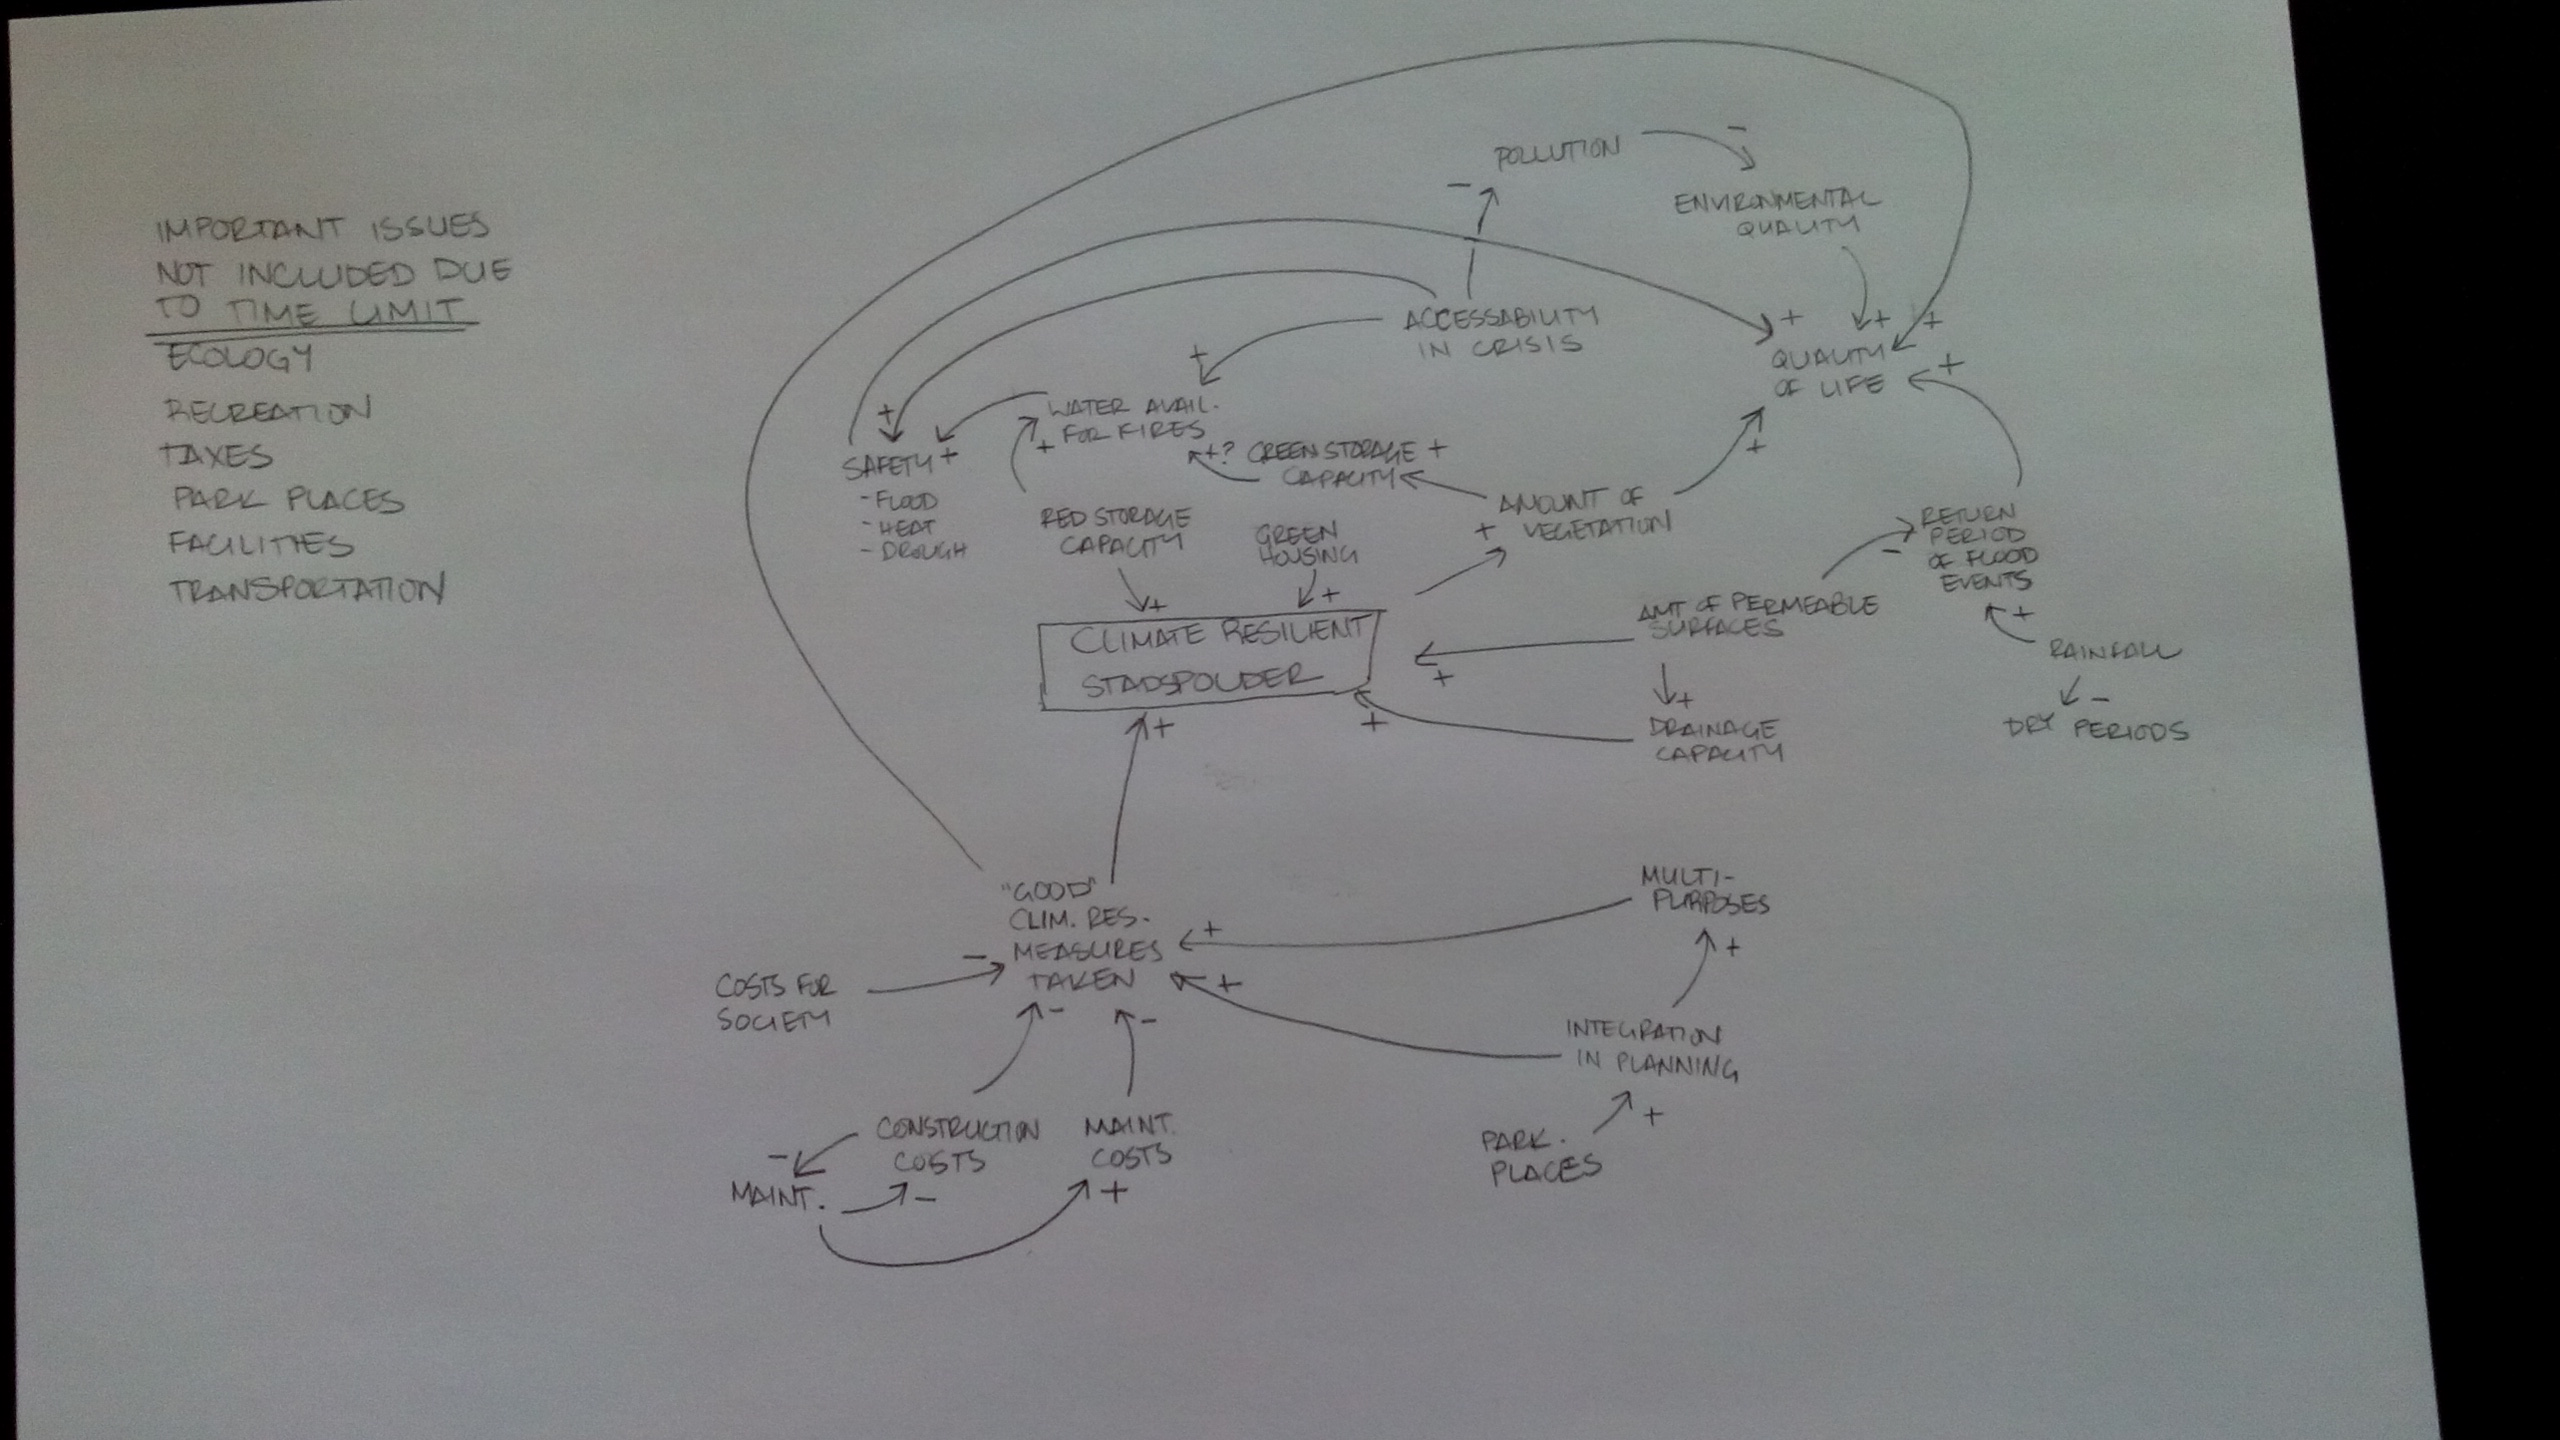
\includegraphics[width=\textwidth]{../cl1.png}
  \caption{Causal loop diagram 1}
  \label{fig:cl1}%
\end{sidewaysfigure}

\begin{sidewaysfigure}[ht]
  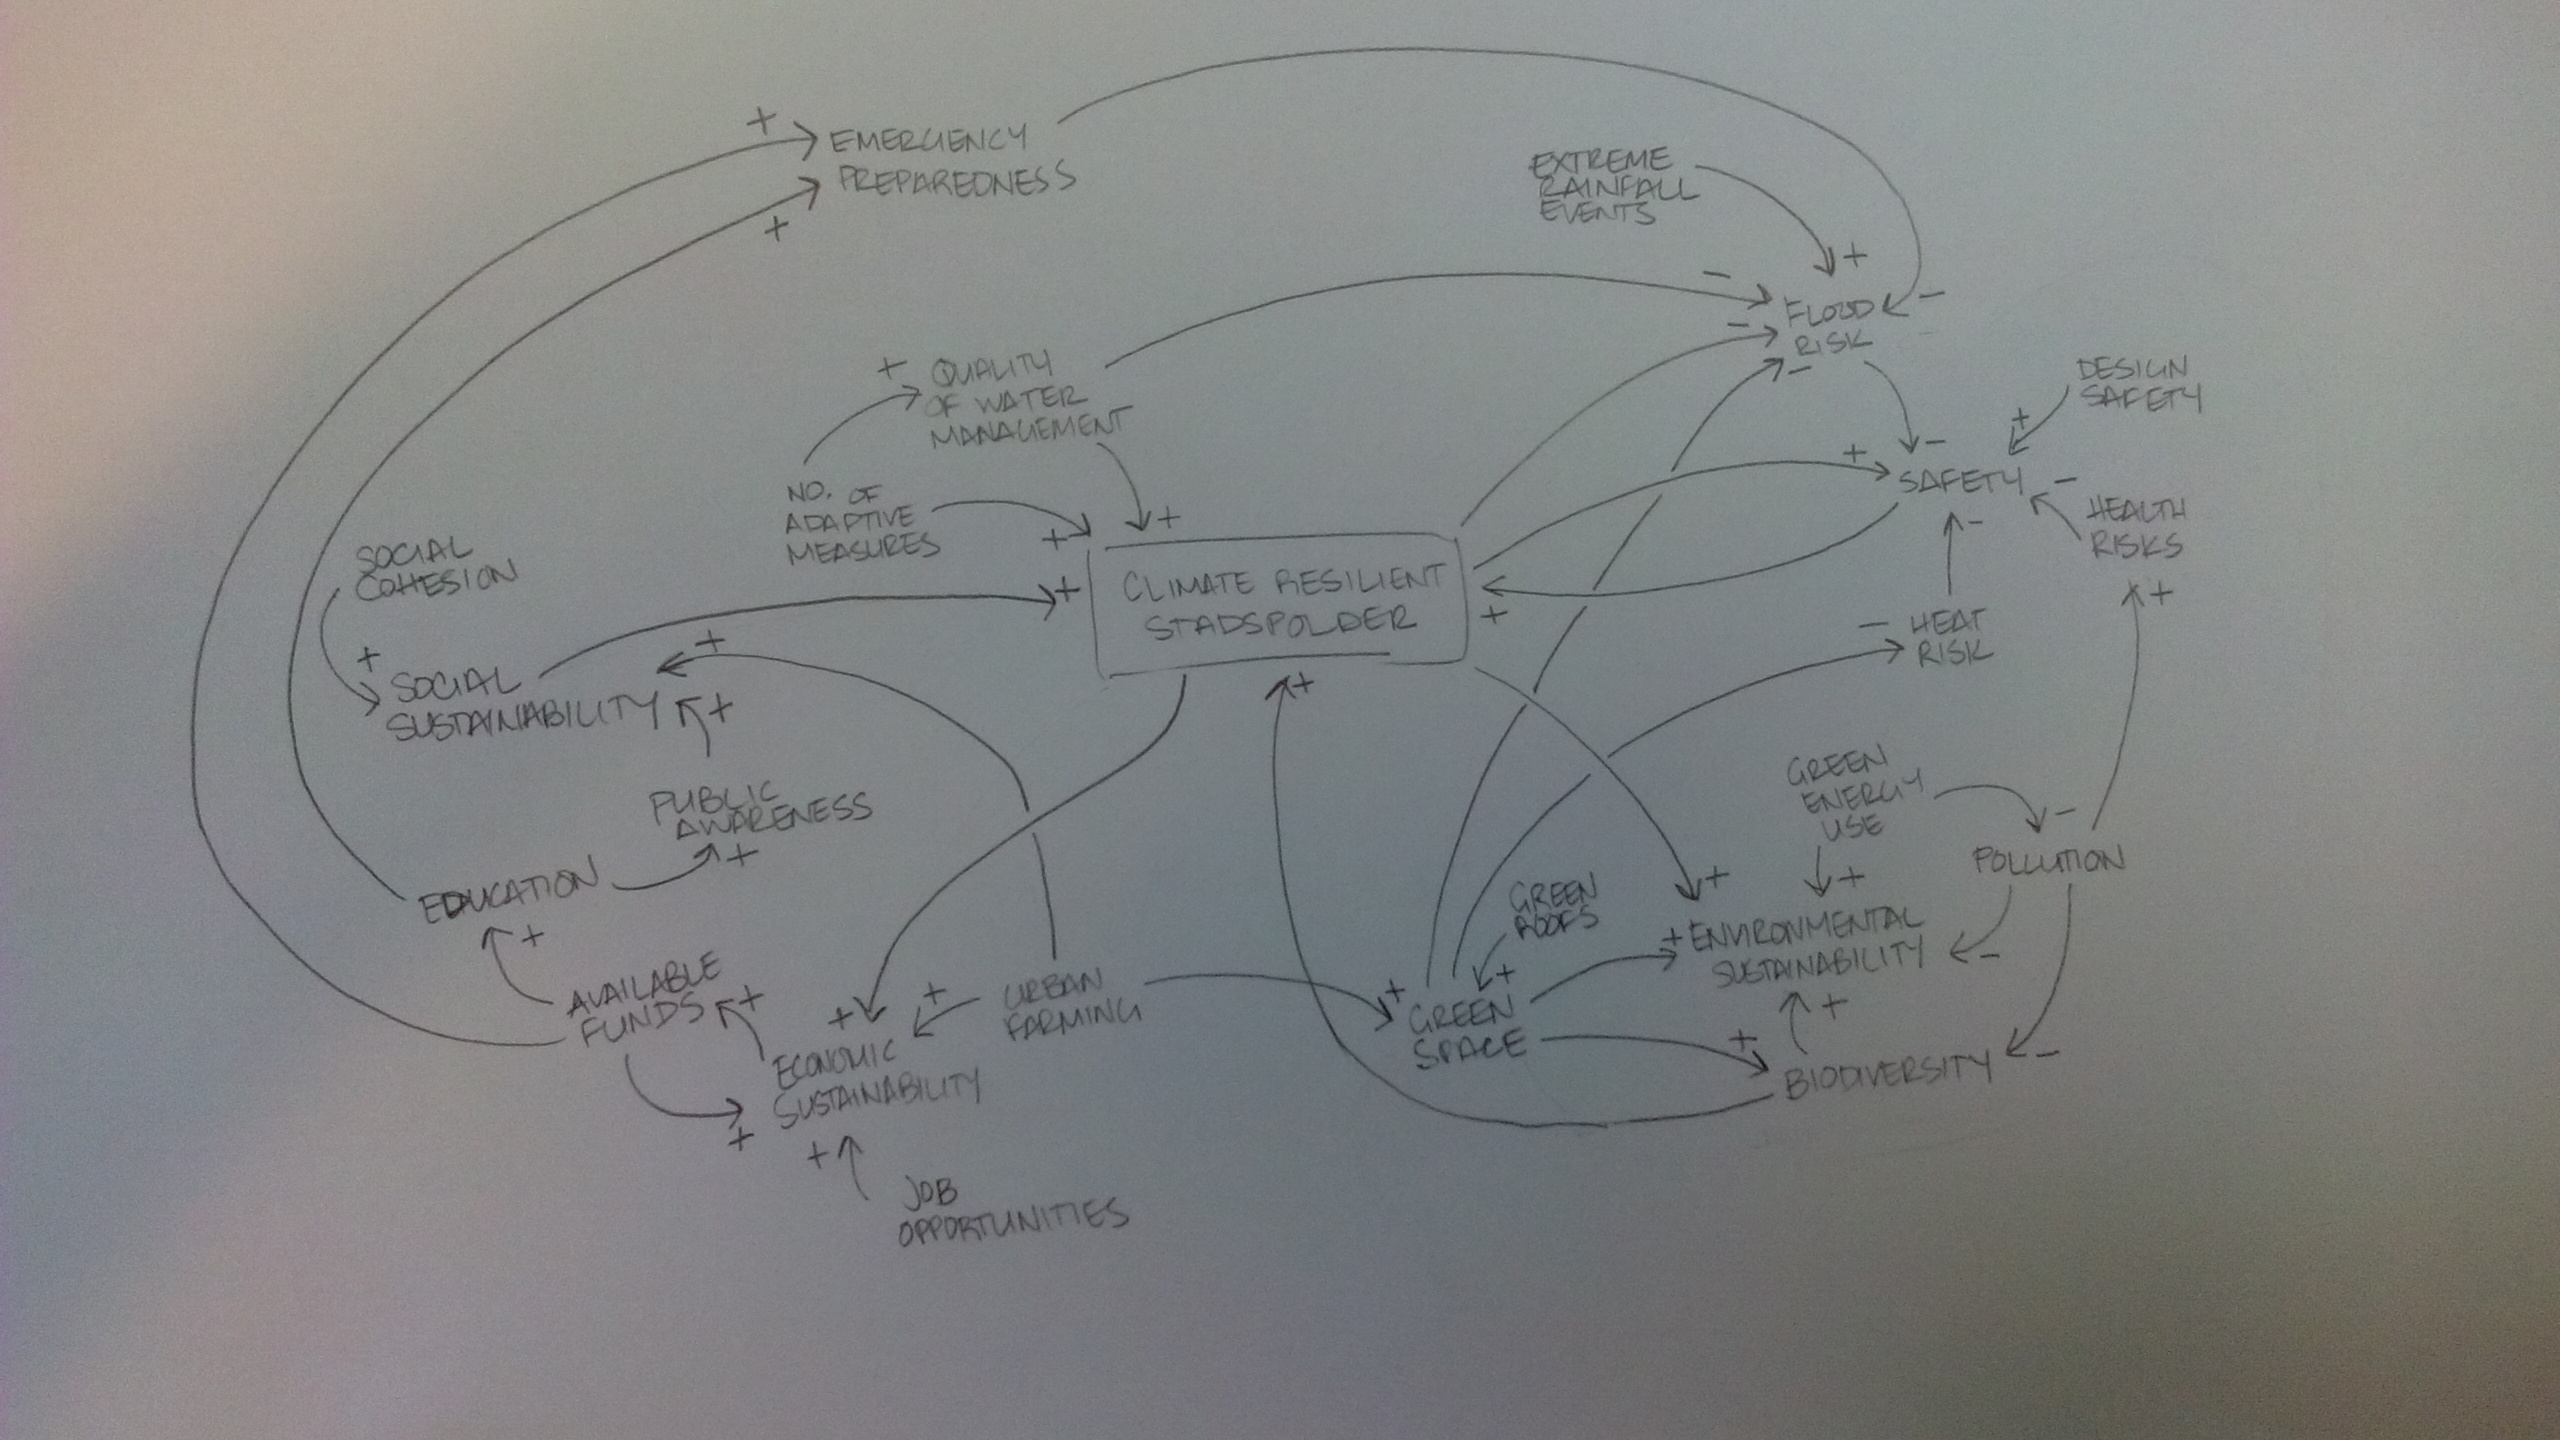
\includegraphics[width=\textwidth]{../cl2.png}
  \caption{Causal loop diagram 2}
  \label{fig:cl2}%
\end{sidewaysfigure}


\end{document}
